\documentclass[12pt]{article}
\usepackage[margin=1in]{geometry}
\usepackage{graphicx}
\usepackage{amsmath, amssymb}
\usepackage{booktabs}
\usepackage{hyperref}
\usepackage{enumitem}
\usepackage{float}
\usepackage{diagbox}
\usepackage{fancyhdr}
\usepackage{bbm}
\usepackage{color}
\usepackage{listings}
\usepackage{caption} 
\usepackage{subcaption}
\usepackage{xcolor}

\pagestyle{fancy}
\fancyhf{}
\rhead{Numerical Methods \& Optimization – ENSIA}
\lhead{Feature Selection with PSO}
\cfoot{\thepage}

\title{
    \vspace{1cm}
    \Huge{\textbf{Feature Selection for Classification using Particle Swarm Optimization (PSO)}}\\
    \vspace{0.5cm}
    \Large{Numerical Methods \& Optimization – ENSIA}
}
\author{
    \large{Project Team:} \\
    \textbf{Bouabdelli Moulay Mohamed - G1} \\
    \textbf{Chaalel Omar Ziyad - G5} \\
    \textbf{Frihaoui Mohammed - G1} \\
    \vspace{0.3cm}
    \normalsize{Supervised by: Dr. Lakehal Soumaya}
}
\date{\today}

\begin{document}

\maketitle
\thispagestyle{empty}
\newpage

\tableofcontents
\newpage

% ==================
\section{Introduction}

Feature selection is a very popular data pre-processing technique that simplifies models by removing unimportant or redundant features, making them more interpretable and stable in learning in some cases. The chosen subset can then be tested against a fitness function to assess its optimality.

As the number of dimensions (features) increase, finding said optimal subset through search becomes an intractable problem \cite{kohavi1997wrappers}. And many problems that are related or can be reduced to this problem are NP hard problems\cite{blum1992npcomplete}.

The dataset we will use for this project is the \textit{Breast Cancer Wisconsin (Diagnostic) Dataset} first introduced in \cite{Street1993NuclearFE} obtained from the \textit{scikit-learn API}. It contains 30 features related to breast cancer diagnoses, where the goal is to predict whether a tumor is malignant or benign.

Particle Swarm Optimization (PSO) would be beneficial in this case to select a near-optimal subset of features that most impact the perfect classifier decisions without having to explore an intractable search space.

% ==================
\section{Problem Definition and Mathematical Model}
\subsection{Objective}
The objective is to find the optimal subset of features that results in the highest performance of a classifier. Performance measure is \textit{ accuracy} defined as :
$$ \text{Accuracy} = \frac{TP + TN}{TN + TP + FP + FN} $$

where \{TP, TN, FP, FN\} are the components of a binary classifier confusion matrix.

\subsection{Mathematical Formulation}
Let:
\begin{itemize}
    \item \( n \): number of features.
    \item \( x = (x_1, x_2, \dots, x_n) \in \{0, 1\}^n \): binary mask vector indicating selected features.
    \item \( f(x) \): classification accuracy of model using features selected by \( x \).
\end{itemize}
\textbf{Optimization Problem:}
\[
\max_{x \in \{0,1\}^n} f(x)
\]
\textbf{Constraints:} Optional constraint to limit number of selected features:
\[
\sum_{i=1}^n x_i \leq k \quad \text{(optional)}
\]

Alternatively, we will reformulate the problem slightly into minimization by using the fact that \[ \max_{x \in \{0,1\}^n} f(x) \leq 1 \] and factoring in the penalty from the constraint as follows :
$$ \min_{x \in \{0,1\}^n} S(x) $$
Where : 
$$ S(x) =  1 - f(x) + 0.01\cdot \frac{\text{num\_features(x)}}{\text{total\_features}} \cdot \mathbbm{1}_{num\_features(x) > 20}(x) $$

\subsubsection*{Problem Complexity Analysis}
The feature selection task described above is a form of \textit{subset selection} over \( n \) binary decision variables. Since the number of possible subsets is \( 2^n \), the search space grows exponentially with the number of features. This combinatorial explosion renders exhaustive search infeasible for even moderately sized \( n \).

Furthermore, the general subset selection problem for optimizing a classification performance metric (such as accuracy) is known to be NP-Hard \cite{blum1992npcomplete}. This is because evaluating each subset requires training and validating a classifier, and no known polynomial-time algorithm can guarantee the global optimum. Thus, heuristic and metaheuristic methods like Particle Swarm Optimization (PSO) are commonly employed to explore this space efficiently.

% ==================
\section{Particle Swarm Optimization (PSO)}
\subsection{PSO Overview}
Particle Swarm Optimization (PSO) is a computational method designed to optimize problems by iteratively refining candidate solutions with respect to a specified measure of quality while requiring minimal parametrization\cite{pereira2011pso}.

This paradigm was initially introduced by James Kennedy and Russel Ebhart in 1995\cite{pereira2011pso}, it is inspired by \textit{Swarm Intelligence} which is a social behavioral pattern known in many animals that live in cooperative societies particularly fish and birds flocking \cite{ChengS2018swarm}.

The algorithm can be thought of as an analogy to birds flocking in the following manner, a bird flock (swarm of particles constituting a set of states) travels around its habitat (the problem state space) using group and individual learning looking for a place for them to settle down in which shelters them and provides them with food ..., the latter can be abstracted to the notion of a \textit{fitness function} which the algorithm optimizes \cite{sengupta2018}.

\subsection{Binary PSO}

Binary Particle Swarm Optimization (BPSO) is a variant of the standard PSO algorithm adapted for discrete or binary search spaces. It is particularly used for subset selection problems, where the solution space consists of binary vectors indicating the inclusion (1) or exclusion (0) of features.

In BPSO, the position of each particle is represented by a binary vector, and the velocity reflects the probability of a bit being 1. Unlike standard PSO, which updates positions based on continuous values, BPSO uses a probabilistic mechanism to map the continuous function to a binary output based on a threshold, which reduces the problem to searching in a finite space which can in theory speed up the convergence of particles \cite{zain2014bpso}.

\begin{itemize}
    \item \textbf{Velocity update formula}:
    \[
    v_i(t+1) = w \cdot v_i(t) + c_1 \cdot r_1 \cdot (p_i - x_i(t)) + c_2 \cdot r_2 \cdot (g - x_i(t))
    \]
    where:
    \begin{itemize}
        \item \( v_i(t) \): velocity of particle \(i\) at time \(t\)
        \item \( x_i(t) \): current position of particle \(i\)
        \item \( p_i \): best known position of particle \(i\) (personal best)
        \item \( g \): global best position among all particles
        \item \( r_1, r_2 \sim U(0, 1) \): random numbers
        \item \( w \): inertia weight
        \item \( c_1, c_2 \): cognitive and social coefficients
    \end{itemize}
    
    \item \textbf{Sigmoid transfer function} (used to squash velocity into a probability range [0,1]):
    \[
    S(v_i) = \frac{1}{1 + e^{-v_i}}
    \]
    
    \item \textbf{Position update rule} (based on probability output by the sigmoid):
    \[
    x_{i} = 
    \begin{cases}
    1, & \text{if } r < S(v_i) \\
    0, & \text{otherwise}
    \end{cases}
    \quad \text{where } r \sim U(0, 1)
    \]
\end{itemize}


% ==================
\section{Implementation Details}
\subsection{Programming Environment}
\begin{itemize}
    \item Language: Python
    \item Libraries: NumPy (Matrix-Like Data Manipulations), scikit-learn (Dataset, Classifier \& Metrics).
\end{itemize}
\textit{Why Python ?} Python allows for faster implementations and testing of ideas due to its high level nature, abstracting significant boilerplate code and memory management that would otherwise be accounted for in many other technologies like C++ or MATLAB. 

Furthermore, has a flourishing ecosystem of libraries for computation and machine learning in general. And through tools like Cython, Python code can be compiled into C++/C to offload high-performance components, leaving the focus on algorithm design, evaluation and visualization rather than technology dependent optimization tweaks.


\subsection{Fitness Function \& BPSO}
\begin{itemize}
    \item Accuracy of classifier on validation data.
    \item Include penalty for number of selected features to prevent the swarm from favoring solutions with excessive number of features.
    \item We set BPSO to run for 50 iterations with an early stopping patience parameter set to 20, i.e if the algorithm does not find any improvement 20 iterations in a row, we stop it.
    \item The swarm is set to contain 30 particles.
    \item We use the minimization formulation of the problem and include the penalty as we discussed above, penalty multiplier is set to 0.01.
    \item All these \textit{hyper-parameters} can be subject to fine tuning through learning in a continuous state space via gradient descent.
\end{itemize}

\subsection{Classifier Used}
\begin{itemize}
    \item Random Forest with 10 estimators each using the \textit{Gini} impurity as the splitting criterion.
\end{itemize}
\newpage
% ==================
\section{Results and Analysis}

In this section, we present the results obtained from applying Particle Swarm Optimization (PSO) for feature selection and its effect on classifier performance. We provide an in-depth analysis of the optimization process, the performance metrics, and convergence behavior. Additionally, we include visualizations and tables to better illustrate the outcomes.

\subsection{Performance Metrics}

The optimization process led to significant improvements in the classification performance. Here are the key performance metrics:

\begin{itemize}
    \item \textbf{Best Accuracy Achieved}: 0.9942 (99.42\%)
    \item \textbf{Number of Iterations}: 45
    \item \textbf{Optimization Time}: 17.61 seconds
    \item \textbf{Early Stopping}: Triggered due to lack of further improvement
\end{itemize}

The achieved accuracy of 99.42\% indicates that the selected subset of features was highly discriminative, leading to excellent model performance on the dataset.

\subsection{Convergence Behavior}

The convergence curve shows how the accuracy of the classifier evolved over the iterations of the PSO algorithm. Below is the plot representing the accuracy across iterations:

\begin{figure}[H]
    \centering
    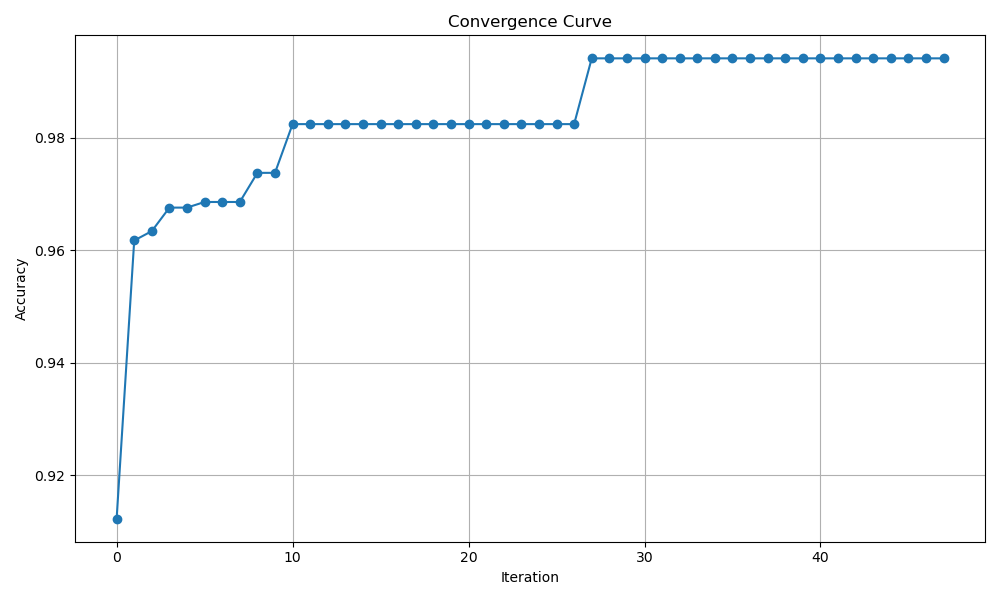
\includegraphics[width=0.85\textwidth]{convergence_curve.png}
    \caption{Convergence curve showing accuracy over iterations. The accuracy increases rapidly during the early iterations, reaching a plateau around iteration 28. This plateau reflects the algorithm’s convergence to a local or global optimum.}
    \label{fig:convergence}
\end{figure}

The \textbf{convergence curve} (Figure \ref{fig:convergence}) shows rapid improvements in accuracy during the initial iterations, indicating that the swarm was effectively exploring the feature space. The accuracy then stabilizes after iteration 28, which suggests that the optimization process has found a near-optimal subset of features. Early stopping was triggered after 45 iterations, signaling that further exploration would not yield significant improvements.

\subsection{Interpretation of Feature Selection Frequencies}

We also analyzed the frequency with which individual features were selected across the particles in the swarm. This is visualized in the following bar chart:

\begin{figure}[H]
    \centering
    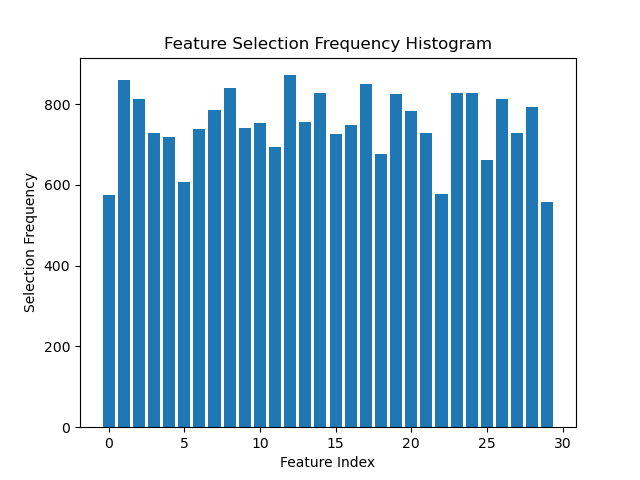
\includegraphics[width=0.75\textwidth]{feature_selection_frequency.png}
    \caption{Bar chart of feature selection frequency across particles.}
    \label{fig:feature_freq}
\end{figure}

\subsection{Feature Selection Frequency}

The feature selection frequency plot (Figure \ref{fig:feature_freq}) reveals that the distribution of feature selections is nearly uniform, with slight fluctuations in the selection frequency of individual features. This indicates that the PSO algorithm is efficiently exploring the feature set space, taking most features into consideration for the training, this might also suggest that no one feature is significantly more dominant than the others in influencing the model decisions. 

\subsection{Comparison of Accuracy with Different Swarm Sizes and Iteration Counts}

The table below shows the performance of the PSO algorithm with varying swarm sizes and iteration counts. We present the best achieved accuracy for different combinations of these parameters:

\begin{table}[H]
\centering
\caption{Best Accuracy Achieved for Different Combinations of Iterations and Swarm Sizes}
\label{tab:accuracy_comparison}
\begin{tabular}{|c|c|c|c|c|}
\hline
\diagbox{Iterations}{Swarm Size} & \textbf{10} & \textbf{25} & \textbf{50} & \textbf{100} \\
\hline
\textbf{10}   & 0.9766 & 0.9766 & 0.9766 & 0.9796 \\
\textbf{20}   & 0.9883 & 0.9825 & 0.9942 & 0.9883 \\
\textbf{50}   & 0.9883 & 0.9942 & 1.0000 & 1.0000 \\
\textbf{100}  & 0.9942 & 0.9883 & 0.9942 & 1.0000 \\
\hline
\end{tabular}
\end{table}

The \textbf{accuracy comparison table} (Table \ref{tab:accuracy_comparison}) demonstrates that increasing both the swarm size and the number of iterations leads to higher classification accuracy. The highest accuracy (1.0000) was achieved when the swarm size was 50 or 100, and the number of iterations was set to 50 or 100. This shows that larger swarm sizes enhance the exploration capabilities, while more iterations improve convergence towards the optimal solution which comes at the expense of having a very long running time but we can also see that our chosen configuration (50 iterations, 30 particles) achieves a good trade-off between accuracy and runtime.

\subsection{Optimization Time and Efficiency}

The optimization time of 17.61 seconds indicates that PSO can provide near-optimal feature subsets in a relatively short period. The effectiveness of early stopping (which halted the algorithm after 45 iterations) also contributed to this efficiency, preventing unnecessary computation.

---

\subsection{Summary of Observations}

\begin{itemize}
    \item \textbf{Early Exploration and Rapid Convergence}: The PSO algorithm showed rapid improvements in accuracy during the initial iterations, effectively exploring the feature space before converging to an optimal or near-optimal subset of features.
    \item \textbf{Impact of Swarm Size and Iterations}: Larger swarm sizes and more iterations consistently led to better performance, with 50 or more particles and at least 50 iterations achieving near-perfect classification accuracy.
    \item \textbf{Optimization Time}: The process completed in under 20 seconds, making PSO a relatively fast method for feature selection, especially with early stopping incorporated.
\end{itemize}

By restructuring the results and analysis section with comments on each figure and table, we now have a clear narrative that explains the significance of each visualization, the relationship between the swarm size, iterations, and classifier performance, and the efficiency of the PSO algorithm.



% ==================
\section{Challenges}
\textbf{Sub-optimal Convergence} : BPSO is prone to converging too quickly to local optima and the search space is saturated with plateaus occurring in a huge variety of subsets which makes convergence to the global optimum less and less likely.

\textbf{Computational Time} : In a world where decisions are taken in split seconds, the algorithm running time is impacted by the major time consuming factor in the optimization pipeline which is evaluating the fitness function, so better implementations which could support parallelism should be considered.

\textbf{Parameter Sensitivity} : PSO is notably sensitive to its parameter settings, which significantly impacts its performance in convergence speed and optimality. The main parameters within PSO, such as the inertia weight, acceleration coefficients, and the total number of particles, play critical roles and therefore selecting them is a non trivial task which could also be done through various search mechanisms to avoid all aforementioned problems \cite{mostafa2022convergencepso}.

% ==================
\section{Conclusion}
In this project, we tackled the problem of feature selection for classification tasks using Binary Particle Swarm Optimization (BPSO). By formulating the task as a combinatorial optimization problem, we aimed to find the most informative subset of features from the Breast Cancer Wisconsin Diagnostic Dataset to maximize classification accuracy while minimizing model complexity.

Our results demonstrate that BPSO is an effective and computationally efficient technique for feature selection. It achieved high classification accuracy (up to 99.42\%) within a reasonable time frame and showed strong convergence behavior. We observed that larger swarm sizes and iteration counts led to improved results (100\%), though with increased computational cost.

However, we also encountered several challenges, including sensitivity to the considerable number of hyperparameters, risk of premature convergence, and the high computational cost of evaluating the fitness function. These highlight opportunities for future work, such as:
\begin{itemize}
\item Using adaptive parameter tuning methods to improve convergence.
\item Leveraging parallel computing to reduce runtime.
\item Exploring alternative fitness functions and penalty designs that better balance accuracy and sparsity of feature selection.
\end{itemize}

Overall, our study reaffirms the potential of metaheuristic algorithms like PSO in solving high-dimensional optimization problems, especially in the context of feature selection in machine learning pipelines.

% ==================
\newpage
\section*{Appendix}
\subsection*{Code Snippet: Velocity and Position Update}
\begin{lstlisting}[language=Python, basicstyle=\ttfamily\small]
velocities[i][j] = (w * velocities[i][j] +
                    c1 * r1 * (pbest[i][j] - swarm[i][j]) +
                    c2 * r2 * (gbest[j] - swarm[i][j]))
swarm[i][j] = 1 if random.random() < sigmoid(velocities[i][j]) else 0
\end{lstlisting}
\subsection*{Code Snippet: Minimization Objective Function}
\begin{lstlisting}[language=Python, basicstyle=\ttfamily\small]
acc = accuracy_score(y_test, predictions)
penalty = 0.01 * curr_features / all_features * (curr_features > 20)
score = 1 - acc + penalty
\end{lstlisting}

\subsection*{Full Python Code Repository}
\href{https://github.com/ENSIA-AI/NMO-Alpha-PSO}{GitHub Repository Link}

\newpage
\bibliographystyle{plain}
\bibliography{references}


\end{document}
